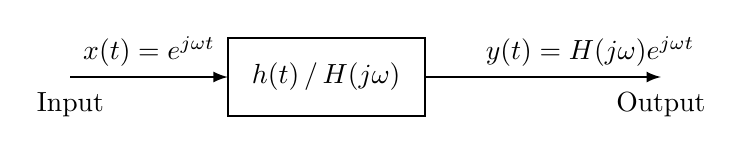
\begin{tikzpicture}[>=latex]
	% Define important coordinates
	\coordinate (input) at (0,0);
	\coordinate (block_left) at (2,-0.5);
	\coordinate (block_right) at (4.5,0.5);
	\coordinate (system_center) at (3.25,0); % Slightly left for visual balance
	\coordinate (output) at (7.5,0);
	
	% Draw main system block (wider, taller)
	\draw[thick] (block_left) rectangle (block_right);
	\node at (system_center) {$h(t)\,/\,H(j\omega)$};
	
	% Arrows and input/output signals
	\draw[->, thick] (input) -- (2,0) node[midway, above] {$x(t) = e^{j\omega t}$};
	\draw[->, thick] (4.5,0) -- (output) node[pos=0.7, above] {$y(t) = H(j\omega)e^{j\omega t}$}; % <-- changed pos=0.7
	
	% Labels for input and output
	\node[below=2pt] at (input) {Input};
	\node[below=2pt] at (output) {Output};
\end{tikzpicture}
